\chapter{Manual de Usuario}

\section{Cuadro de Mando General (CMG)}

\textit{Diego's Software \& Systems} se complace en presentarle el simulador de una
Ciudad Deportiva. A grandes rasgos podr\'a observar un comportamiento aleatorio
en cada simulaci\'on con distintas opciones que da a la aplicaci\'on en si, gran
versatilidad y realismo para probar este tipo de entornos.

\begin{figure}[h]
\begin{center}
 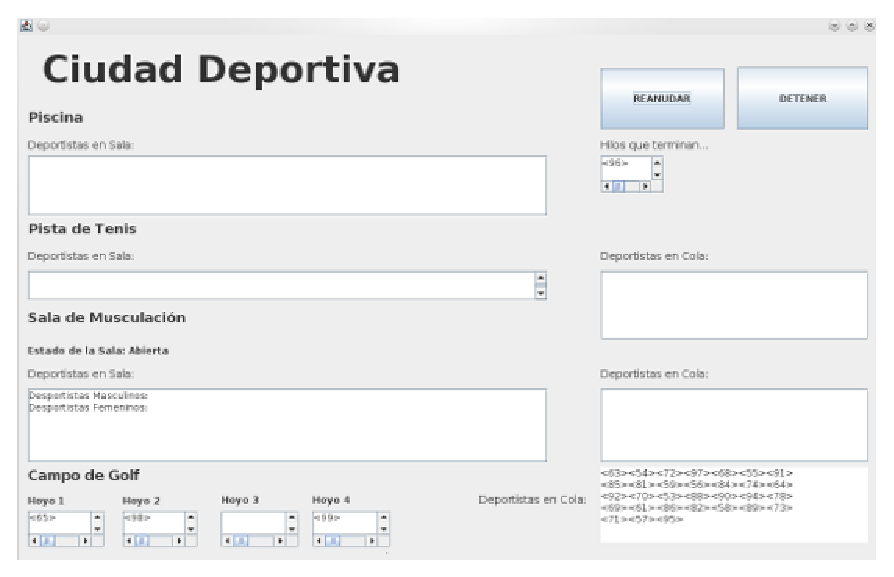
\includegraphics{./images/generalCiudadDeportiva.eps}
 % generalCiudadDeportiva.eps: 0x0 pixel, 300dpi, 0.00x0.00 cm, bb=
\end{center}
\caption{Cuadro de Mando General (CMG).}
\end{figure}


El Cuadro de Mando General se muestra en la Figura 2.1. Diremos que tiene como
funci\'on principal el proporcionar un total control de la ejecuci\'on del
programa. Podr\'a observar d\'onde se encuentra cada doportista y como cumple
sus objetivos, desde que acude a la Piscina hasta que finaliza su ciclo. 

\begin{figure}[h]
\begin{center}
 
\includegraphics{./images/botonReanudar.eps}
 % botonReanudar.eps: 0x0 pixel, 300dpi, 0.00x0.00 cm, bb=
\end{center}
\caption{Vista detallada del bot\'on Reanudar del CMG.}
\end{figure}


\begin{figure}[h]
\begin{center}
 
\includegraphics{./images/botonDetener.eps}
 % botonDetener.eps: 0x0 pixel, 300dpi, 0.00x0.00 cm, bb=
\end{center}
\caption{Vista detallada del bot\'on Detener del CMG.}
\end{figure}


\begin{figure}[h]
\begin{center}
 
\includegraphics{./images/findeHilos.eps}
 % findeHilos.eps: 0x0 pixel, 300dpi, 0.00x0.00 cm, bb=
\end{center}
\caption{Vista detallada la finalizaci\'on de la actividad de un deportista.}
\end{figure}







